\begin{tikzpicture}
    \begin{axis}[
        xlabel=Amostras,
        ylabel=Concentra��es,
        title=RMSEP com RLM para o Mn,
        legend pos=north east,
        grid=major,
    ]
    \addplot table[x index=0, y index=1, col sep=space] {tex/dados_colunas.txt};
    \legend{Conc. predita}
    \end{axis}
\end{tikzpicture}


\begin{tikzpicture}
    \begin{axis}[
        xlabel=Amostras,
        ylabel=Concentra��es,
        title=RMSEP com RLM para o Mn,
        legend pos=north east,
        grid=major,
    ]
    \addplot[smooth] table[x index=0, y index=1, col sep=space] {tex/dados_colunas.txt};
    \legend{Conc. predita}
    \end{axis}
\end{tikzpicture}


\begin{tikzpicture}
    \begin{axis}[
        xlabel=Amostras,
        ylabel=Concentra��es,
        title=RMSEP com RLM para o Mn,
        legend pos=north east,
        grid=major,
    ]
    \addplot[mark=none,line width=1.5pt] table[x index=0, y index=1, col sep=space] {tex/dados_colunas.txt};
    \legend{Conc. predita}
    \end{axis}
\end{tikzpicture}

\begin{tikzpicture}
    \begin{axis}[
        xlabel=Amostras,
        ylabel=Concentra��es,
        title=RMSEP com RLM para o Mn,
        legend pos=north east,
        grid=major,
    ]
    \addplot[
        mark=none,           % Remove os marcadores
        line width=1.5pt,     % Espessura da linha
        color=red             % Cor da linha (vermelho)
    ] table[x index=0, y index=1, col sep=space] {tex/dados_colunas.txt};
    \legend{Conc. predita}
    \end{axis}
\end{tikzpicture}

%----------------------------------------------
\begin{tikzpicture}
\begin{axis}[
    title={RLM-Bagging de Amostras Mangan�s},
    xlabel={Amostras Mangan�s},
    ylabel={Concentra��o},
    xmin=0, xmax=40,
    ymin=0, ymax=5,
    xtick={0,5,10,15,20,25,30,35,40},
    ytick={0,1,2,3,4,5},
    legend pos=north west,
    grid=major,
    grid style=dashed,
]

% Dados observados
\addplot[
    color=blue,
    mark=square,
    ]
    coordinates {
    (5,4)(10,3)(15,2)(20,1)(25,0)(30,1)(35,2)
    };
    \addlegendentry{Conc. esp.}

% Dados preditos (exemplo - ajuste conforme necess�rio)
\addplot[
    color=red,
    mark=o,
    ]
    coordinates {
    (5,3.8)(10,3.1)(15,2.2)(20,1.1)(25,0.2)(30,1.3)(35,2.1)
    };
    \addlegendentry{Conc. pred.}

\end{axis}
\end{tikzpicture}

%-------------------------------------------------
\begin{center}
\begin{minipage}{0.48\textwidth}
\begin{tikzpicture}
\begin{axis}[
    title={Gr�fico 1: Dados Observados},
    xlabel={Amostras Mangan�s},
    ylabel={Concentra��o},
    xmin=0, xmax=40,
    ymin=0, ymax=5,
    xtick={0,5,10,15,20,25,30,35,40},
    ytick={0,1,2,3,4,5},
    legend pos=north west,
    grid=major,
    grid style=dashed,
    width=\textwidth,
]

% Dados observados
\addplot[
    color=blue,
    mark=square,
    ]
    coordinates {
    (5,4)(10,3)(15,2)(20,1)(25,0)(30,1)(35,2)
    };
    \addlegendentry{Conc. esp.}

\end{axis}
\end{tikzpicture}
\end{minipage}
\hfill
\begin{minipage}{0.48\textwidth}
\begin{tikzpicture}
\begin{axis}[
    title={Gr�fico 2: Dados Preditos},
    xlabel={Amostras Mangan�s},
    ylabel={Concentra��o},
    xmin=0, xmax=40,
    ymin=0, ymax=5,
    xtick={0,5,10,15,20,25,30,35,40},
    ytick={0,1,2,3,4,5},
    legend pos=north west,
    grid=major,
    grid style=dashed,
    width=\textwidth,
]

% Dados preditos
\addplot[
    color=red,
    mark=o,
    ]
    coordinates {
    (5,3.8)(10,3.1)(15,2.2)(20,1.1)(25,0.2)(30,1.3)(35,2.1)
    };
    \addlegendentry{Conc. pred.}

\end{axis}
\end{tikzpicture}
\end{minipage}
\end{center}

%----------------------------------------------------
\begin{center}
\begin{minipage}{0.48\textwidth}
\begin{tikzpicture}
\begin{axis}[
    title={RLM-Bagging de Amostras Mangan�s (Esquerda)},
    xlabel={Amostras Mangan�s},
    ylabel={Concentra��o},
    xmin=0, xmax=40,
    ymin=0, ymax=5,
    xtick={0,5,10,15,20,25,30,35,40},
    ytick={0,1,2,3,4,5},
    legend pos=north east, %north west
    grid=major,
    grid style=dashed,
    width=\textwidth,
]

% Dados observados
\addplot[
    color=blue,
    mark=square,
    ]
    coordinates {
    (5,4)(10,3)(15,2)(20,1)(25,0)(30,1)(35,2)
    };
    \addlegendentry{Conc. esp.}

% Dados preditos
\addplot[
    color=red,
    mark=o,
    ]
    coordinates {
    (5,3.8)(10,3.1)(15,2.2)(20,1.1)(25,0.2)(30,1.3)(35,2.1)
    };
    \addlegendentry{Conc. pred.}

\end{axis}
\end{tikzpicture}
\end{minipage}
\hfill
\begin{minipage}{0.48\textwidth}
\begin{tikzpicture}
\begin{axis}[
    title={RLM-Bagging de Mangan�s (Direita)},
    xlabel={Amostras Mangan�s},
    ylabel={Concentra��o},
    xmin=0, xmax=40,
    ymin=0, ymax=5,
    xtick={0,5,10,15,20,25,30,35,40},
    ytick={0,1,2,3,4,5},
    legend pos=north east,
    grid=major,
    grid style=dashed,
    width=\textwidth,
]

% Dados observados
\addplot[
    color=blue,
    mark=square,
    ]
    coordinates {
    (5,4)(10,3)(15,2)(20,1)(25,0)(30,1)(35,2)
    };
    \addlegendentry{Conc. esp.}

% Dados preditos
\addplot[
    color=red,
    mark=o,
    ]
    coordinates {
    (5,3.8)(10,3.1)(15,2.2)(20,1.1)(25,0.2)(30,1.3)(35,2.1)
    };
    \addlegendentry{Conc. pred.}

\end{axis}
\end{tikzpicture}
\end{minipage}
\end{center}

%---------------------------------------------
\begin{tikzpicture}
    \begin{axis}[
        xlabel=Amostras,
        ylabel=Concentra��es,
        title=RMSEP com RLM para o Mn,
        legend pos=north east,
        grid=major,
    ]
    % Linha vermelha (dados originais)
    \addplot[
        mark=none,
        %line width=0.5pt,
        color=red
    ] table[x index=0, y index=1, col sep=space] {tex/dados_colunas.txt};
    
    % Nova linha azul (dados_testes.txt)
    \addplot[
        mark=none,
        %line width=0.5pt,
        color=blue
    ] table[x index=0, y index=1, col sep=space] {tex/dados_testes.txt};
    
    \legend{Conc. predita, Conc. esperada}
    \end{axis}
\end{tikzpicture}
%-------------------------------------------
\begin{figure}[htbp]
\centering
\caption{RMSEP com RLM para Mn e Fe.}
% Gr�fico da esquerda
\begin{minipage}{0.48\textwidth}
\begin{tikzpicture}
    \begin{axis}[
        xlabel=Amostras,
        ylabel=Concentra��es,
        title=RMSEP com RLM para o Mn (1),
        legend pos=north east,
        grid=major,
        width=\textwidth
    ]
    \addplot[mark=none, color=red] table[x index=0, y index=1, col sep=space] {tex/dados_colunas.txt};
    \addplot[mark=none, color=blue] table[x index=0, y index=1, col sep=space] {tex/dados_testes.txt};
    \legend{Conc. predita, Conc. esperada}
    \end{axis}
\end{tikzpicture}
\end{minipage}
\hfill
% Gr�fico da direita
\begin{minipage}{0.48\textwidth}
\begin{tikzpicture}
    \begin{axis}[
        xlabel=Amostras,
        ylabel=Concentra��es,
        title=RMSEP com RLM para o Fe (2),
        legend pos=north east,
        grid=major,
        width=\textwidth
    ]
    \addplot[mark=none, color=red] table[x index=0, y index=1, col sep=space] {tex/dados_colunas.txt};
    \addplot[mark=none, color=blue] table[x index=0, y index=1, col sep=space] {tex/dados_testes.txt};
    \legend{Conc. predita, Conc. esperada}
    \end{axis}
\end{tikzpicture}
\end{minipage}
\legend{Fonte:~\oautor}
\end{figure}

%---------------------------
\begin{figure}
    \centering
		\caption{RMSEP com RLM para Mn e Fe.}
    \begin{subfigure}{0.45\textwidth}
        \centering
        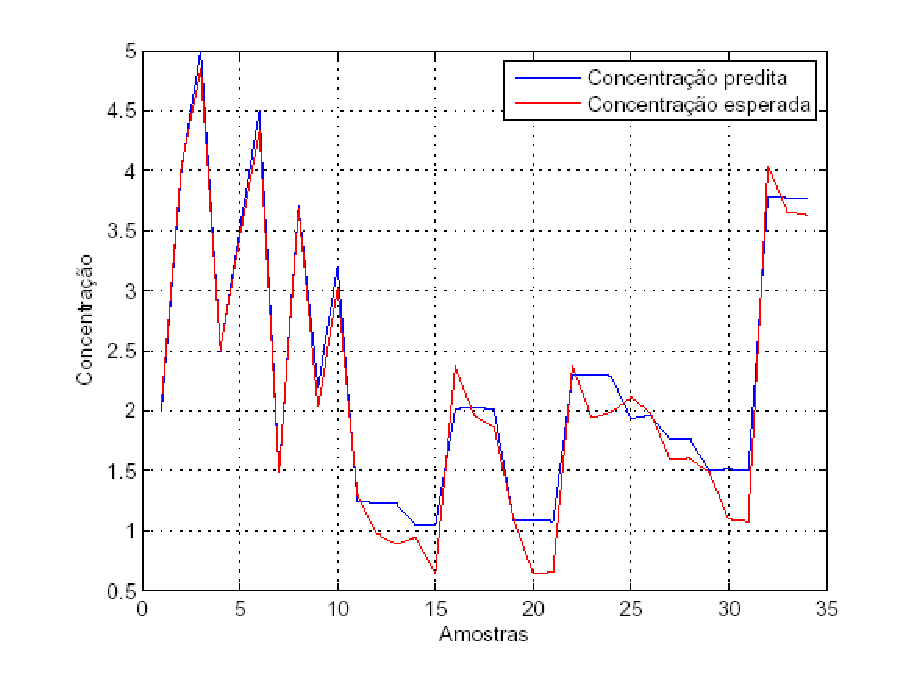
\includegraphics[width=\linewidth]{./outros/fig/Figura41.eps }
        \caption{RMSEP com a RLM para o Mn.}\label{fig:Figura41a}
    \end{subfigure}
    \hfill
    \begin{subfigure}{0.45\textwidth}
        \centering
        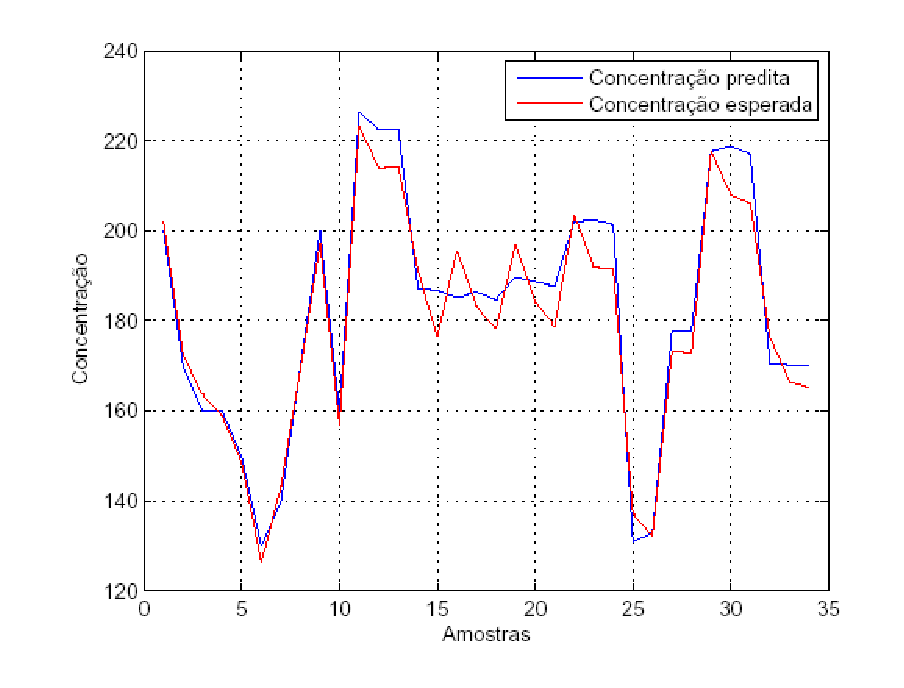
\includegraphics[width=\linewidth]{./outros/fig/Figura41b.eps}
        \caption{RMSEP com RLM para Mn e Fe.}\label{fig:Figura41b}
    \end{subfigure}
\legend{Fonte:~\oautor}
\label{fig:Figura41}
\end{figure}
%------------------------------------------------

\begin{figure}[htbp]
\centering
\caption{RMSEP com RLM para Mn e Fe.}
\label{fig:Figura41}  % Main figure label

% Gr�fico da esquerda (Mn)
\begin{minipage}{0.48\textwidth}
\begin{tikzpicture}
    \begin{axis}[
        xlabel=Amostras,
        ylabel=Concentra��es,
        title=(a) RMSEP com RLM para o Mn,
        legend pos=north east,
        grid=major,
        width=\textwidth
    ]
    \addplot[mark=none, color=red] table[x index=0, y index=1, col sep=space] {tex/dados_colunas.txt};
    \addplot[mark=none, color=blue] table[x index=0, y index=1, col sep=space] {tex/dados_testes.txt};
    \legend{Conc. predita, Conc. esperada}
    \end{axis}
\end{tikzpicture}
\label{fig:Figura41a}  % Left subfigure label
\end{minipage}
\hfill
% Gr�fico da direita (Fe)
\begin{minipage}{0.48\textwidth}
\begin{tikzpicture}
    \begin{axis}[
        xlabel=Amostras,
        ylabel=Concentra��es,
        title=(b) RMSEP com RLM para o Fe,
        legend pos=north east,
        grid=major,
        width=\textwidth
    ]
    \addplot[mark=none, color=red] table[x index=0, y index=1, col sep=space] {tex/dados_colunas.txt};
    \addplot[mark=none, color=blue] table[x index=0, y index=1, col sep=space] {tex/dados_testes.txt};
    \legend{Conc. predita, Conc. esperada}
    \end{axis}
\end{tikzpicture}
\label{fig:Figura41b} % Right subfigure label
\end{minipage}

\legend{Fonte:~\oautor}
\end{figure}
%-------------------SubFigure

